\documentclass[11pt,a4paper]{article}
\usepackage[utf8]{inputenc}
\usepackage[provide=*=spanish]{babel}
\usepackage{graphicx}
\usepackage{geometry}
\usepackage{float}
\usepackage{hyperref}
\usepackage{booktabs}
\geometry{margin=2.5cm}

\begin{document}

\begin{titlepage}
    \centering
    \vspace*{2cm}

    {\Huge \textbf{Universidad Tecnologica de la Mixteca}}\\[2cm]

    {\huge \textbf{Procesamiento de Imágenes de Plantas \\ para la Detección de Plagas}}\\[1.5cm]

    {\Large Primer Parcial: Procesamiento Digital de Imagenes}\\[2.5cm]

    {\large \textbf{Alumno:}}\\
    {\Large Christian Josue Campos Lopez}\\[0.5cm]

    {\large \textbf{Grupo:}}\\
    {\Large [902-A]}\\[2cm]

    {\large \textbf{Profesora:}}\\
    {\Large Dra. Verónica Rodríguez López}\\[2cm]

    \vfill
    {\large \today}
\end{titlepage}

\newpage

%--------------------------------------------------------------
\section{Datos: Descripción del Conjunto de Imágenes}
%--------------------------------------------------------------

El conjunto de imágenes que se utiliza en este proyecto se llama \textit{New Plant Diseases Dataset},
disponible en Kaggle (\url{https://www.kaggle.com/datasets/vipoooool/new-plant-diseases-dataset}).
Contiene miles de fotografías de hojas de plantas, tanto sanas como enfermas,
tomadas en condiciones controladas de laboratorio. Su propósito es servir de base para
sistemas computacionales capaces de identificar qué enfermedad tiene una planta a partir
de sus hojas.

La siguiente tabla resume las características más importantes de las imágenes:

\begin{table}[H]
    \centering
    \renewcommand{\arraystretch}{1.3}
    \begin{tabular}{@{}ll@{}}
        \toprule
        \textbf{Característica} & \textbf{Valor observado} \\ \midrule
        Nombre del conjunto & New Plant Diseases Dataset \\
        Fuente & Kaggle (vipoooool) \\
        Formato de las imágenes & \texttt{.jpg} (JPEG) \\
        Tamaño de las imágenes & 256 $\times$ 256 píxeles \\
        Escala de color & Color (RGB, 3 canales, 24 bits) \\
        Número total de imágenes & 87,900 imágenes \\
        Número de categorías & 38 clases de enfermedades + 1 clase sin etiqueta \\
        Imágenes por categoría & Promedio de $\approx$ 2,100 imágenes por clase \\
        Imágenes de entrenamiento & 70,295 imágenes \\
        Imágenes de validación & 17,572 imágenes \\
        Imágenes de prueba & 33 imágenes \\ \bottomrule
    \end{tabular}
    \caption{Resumen de las características del conjunto de imágenes.}
    \label{tab:dataset_stats}
\end{table}

%--------------------------------------------------------------
\section{Preprocesamiento: Problemas y Soluciones}
%--------------------------------------------------------------

\subsection{Problemas encontrados con las imágenes}

Al revisar las fotografías del conjunto de datos, encontramos cuatro problemas visuales
que dificultan el análisis de las enfermedades:

\begin{itemize}
    \item \textbf{Variación en el número de intensidades (iluminación):} Algunas fotos
    están muy oscuras y otras tienen demasiada luz o brillo. Esto hace que los detalles
    de la hoja sean difíciles de ver con claridad.

    \item \textbf{Imágenes a color y en escala de grises:} Aunque el conjunto está a color,
    ciertas hojas tienen tonos tan pálidos que casi parecen fotografías en blanco y negro.
    Mezclar estos dos tipos de imagen complica el análisis uniforme del conjunto.

    \item \textbf{Variación en el tamaño:} No todas las fotografías tenían el mismo tamaño
    original. Para poder procesarlas todas igual, fue necesario ajustar cada imagen a un
    tamaño estándar de 256 $\times$ 256 píxeles.

    \item \textbf{Ruido en la imagen:} Las fotografías presentan pequeños puntos y manchas
    causados por la propia cámara o por la compresión del archivo. Este ``ruido'' ensucia
    los bordes de la hoja y puede confundirse con síntomas de enfermedad.
\end{itemize}

\subsection{Técnicas aplicadas y flujo de procesamiento}

Para resolver estos problemas, se aplicaron los filtros en el siguiente orden:

\begin{figure}[H]
    \centering
    \fbox{
    \begin{minipage}{0.82\textwidth}
    \centering\vspace{0.5em}
    \textbf{1. Imagen original} \\[0.6em]
    $\downarrow$ \\[0.6em]
    \textbf{2. Filtro de mediana} --- Elimina el ruido sin borrar demasiados detalles \\[0.6em]
    $\downarrow$ \\[0.6em]
    \textbf{3. Ecualización CLAHE} --- Mejora el brillo y contraste en cada zona de la imagen \\[0.6em]
    $\downarrow$ \\[0.6em]
    \textbf{4. Filtro Unsharp} --- Agudiza los bordes y hace los detalles más nítidos \\[0.6em]
    $\downarrow$ \\[0.6em]
    \textbf{5. Resultado final} --- Hoja más limpia, contrastada y enfocada\vspace{0.5em}
    \end{minipage}
    }
    \caption{Diagrama de flujo de las técnicas de preprocesamiento aplicadas.}
    \label{fig:flowchart}
\end{figure}

A continuación se describe qué hace cada técnica en palabras simples:

\begin{enumerate}
    \item \textbf{Filtro de mediana (filtro estadístico para el ruido):} Funciona como un borrador
    muy fino. Quita los puntitos de ruido de la imagen, pero es lo suficientemente cuidadoso para
    \textit{no borrar} los bordes reales de las manchas o lesiones de la hoja.

    \item \textbf{Ecualización CLAHE (transformación de ecualización):} Ajusta el brillo y el
    contraste en zonas pequeñas de la imagen, no en toda la foto a la vez. Así, ilumina las
    partes oscuras sin ``quemar'' las que ya estaban bien iluminadas, logrando una imagen
    más pareja y detallada.

    \item \textbf{Filtro Unsharp (filtro realzante):} Es como ponerle lentes de aumento a la
    imagen. Detecta los bordes y los refuerza para que las venas de la hoja y las manchas
    de la enfermedad se vean con mayor nitidez y definición.

    \item \textbf{Suavizado Gaussiano:} Disminuye variaciones bruscas de intensidad para reducir
    ruido y preparar la imagen antes de aplicar realce. En conjunto, mejora la legibilidad del
    patrón foliar y de las lesiones.
\end{enumerate}

%--------------------------------------------------------------
\section{Resultados y Comparación Visual}
%--------------------------------------------------------------

Se probaron varios filtros de forma individual y en combinación sobre las imágenes del conjunto.
Las siguientes figuras muestran los resultados de aplicar cada técnica:

\clearpage

\begin{figure}[p]
    \centering
    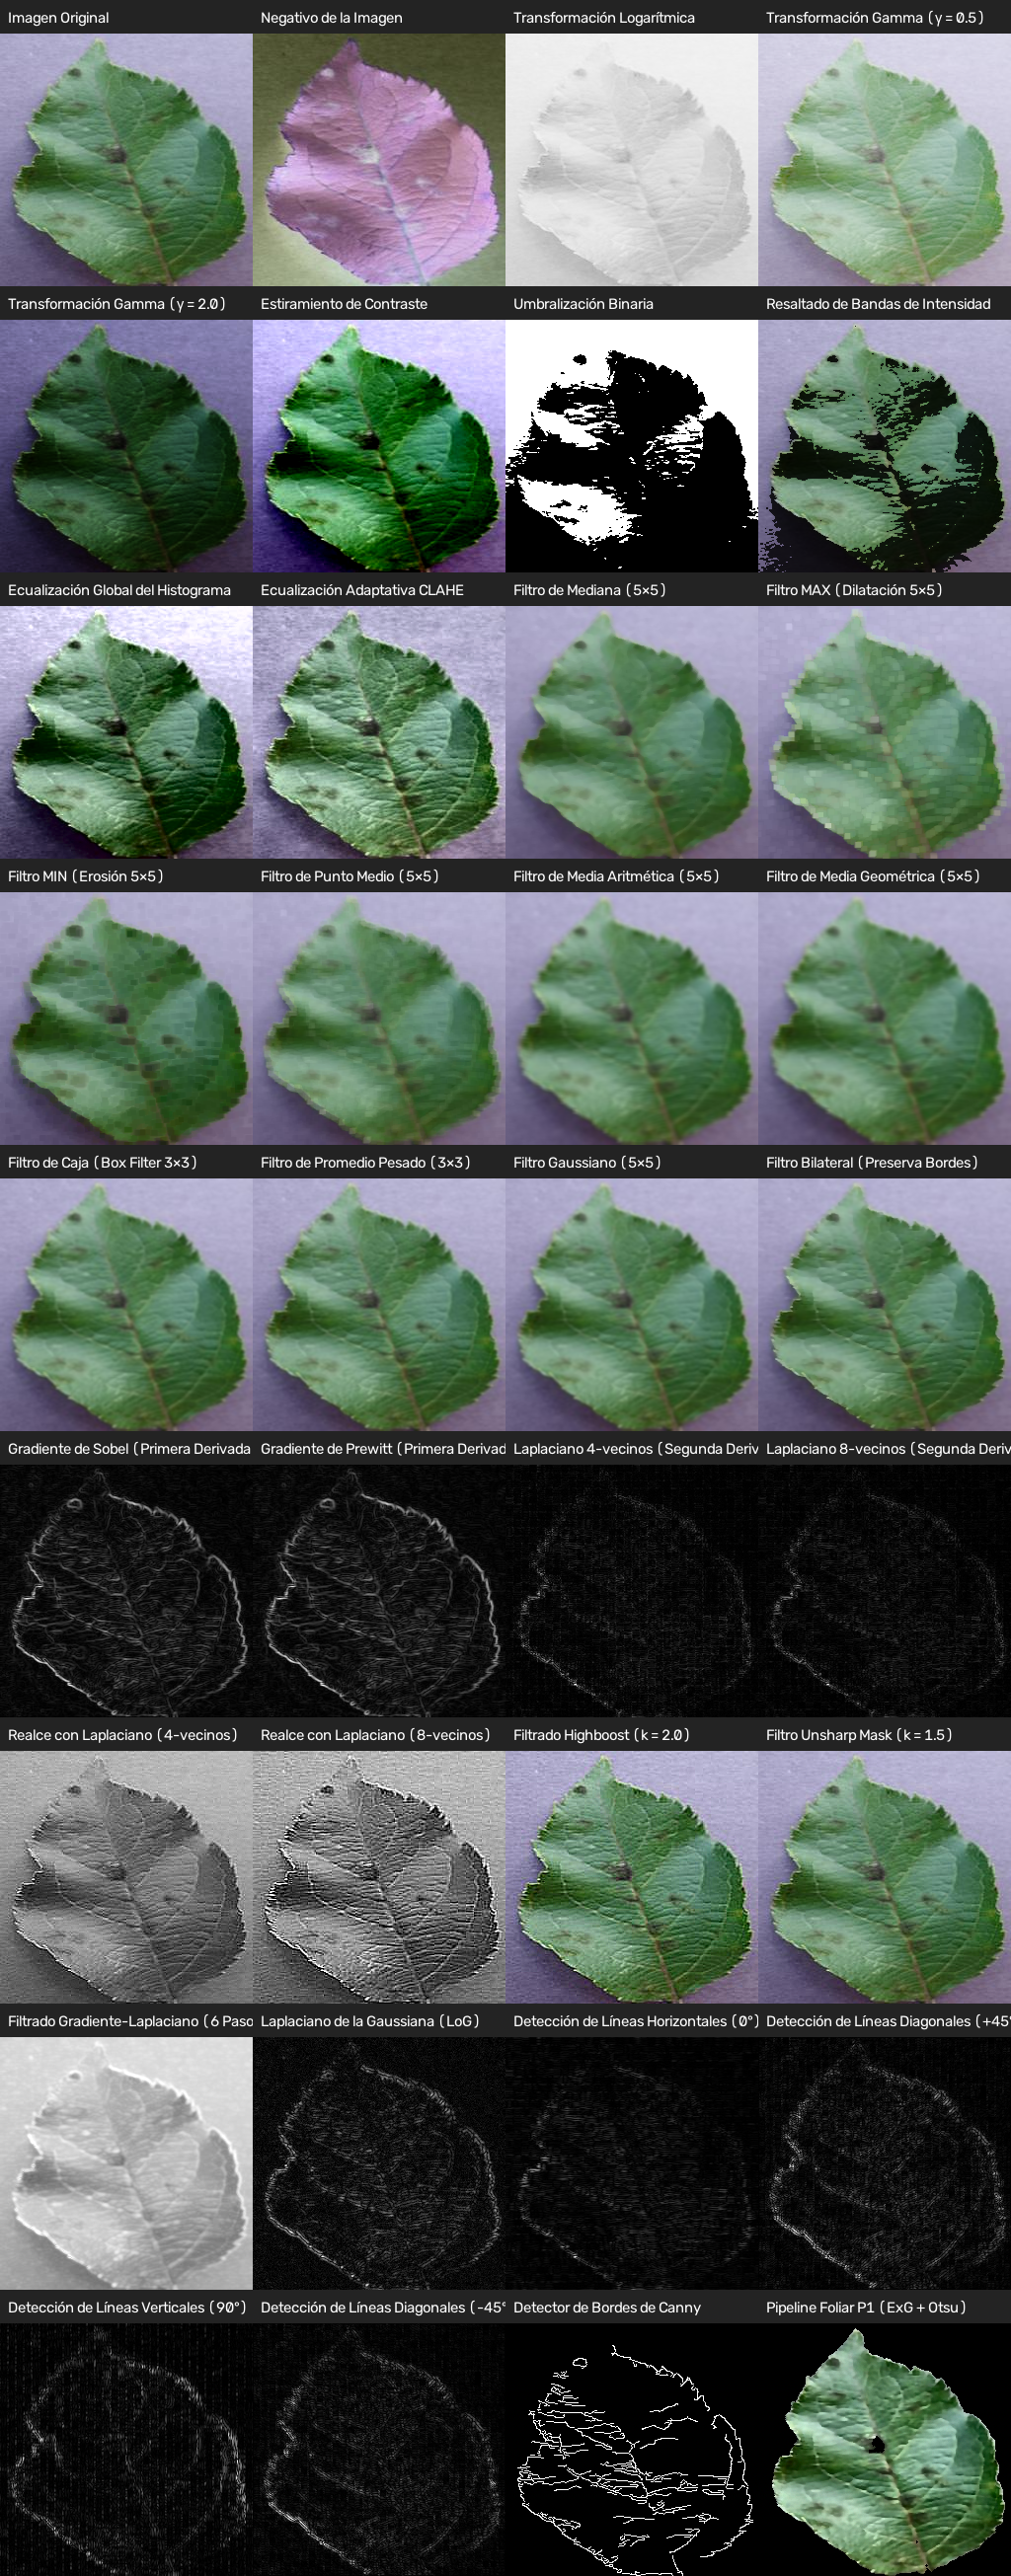
\includegraphics[
        width=\textwidth,
        height=0.72\textheight,
        keepaspectratio
    ]{resultados/filtros_01.png}
    \caption{Comparación de filtros aplicada a la primera imagen de muestra.}
    \label{fig:comparacion1}
\end{figure}

\begin{figure}[p]
    \centering
    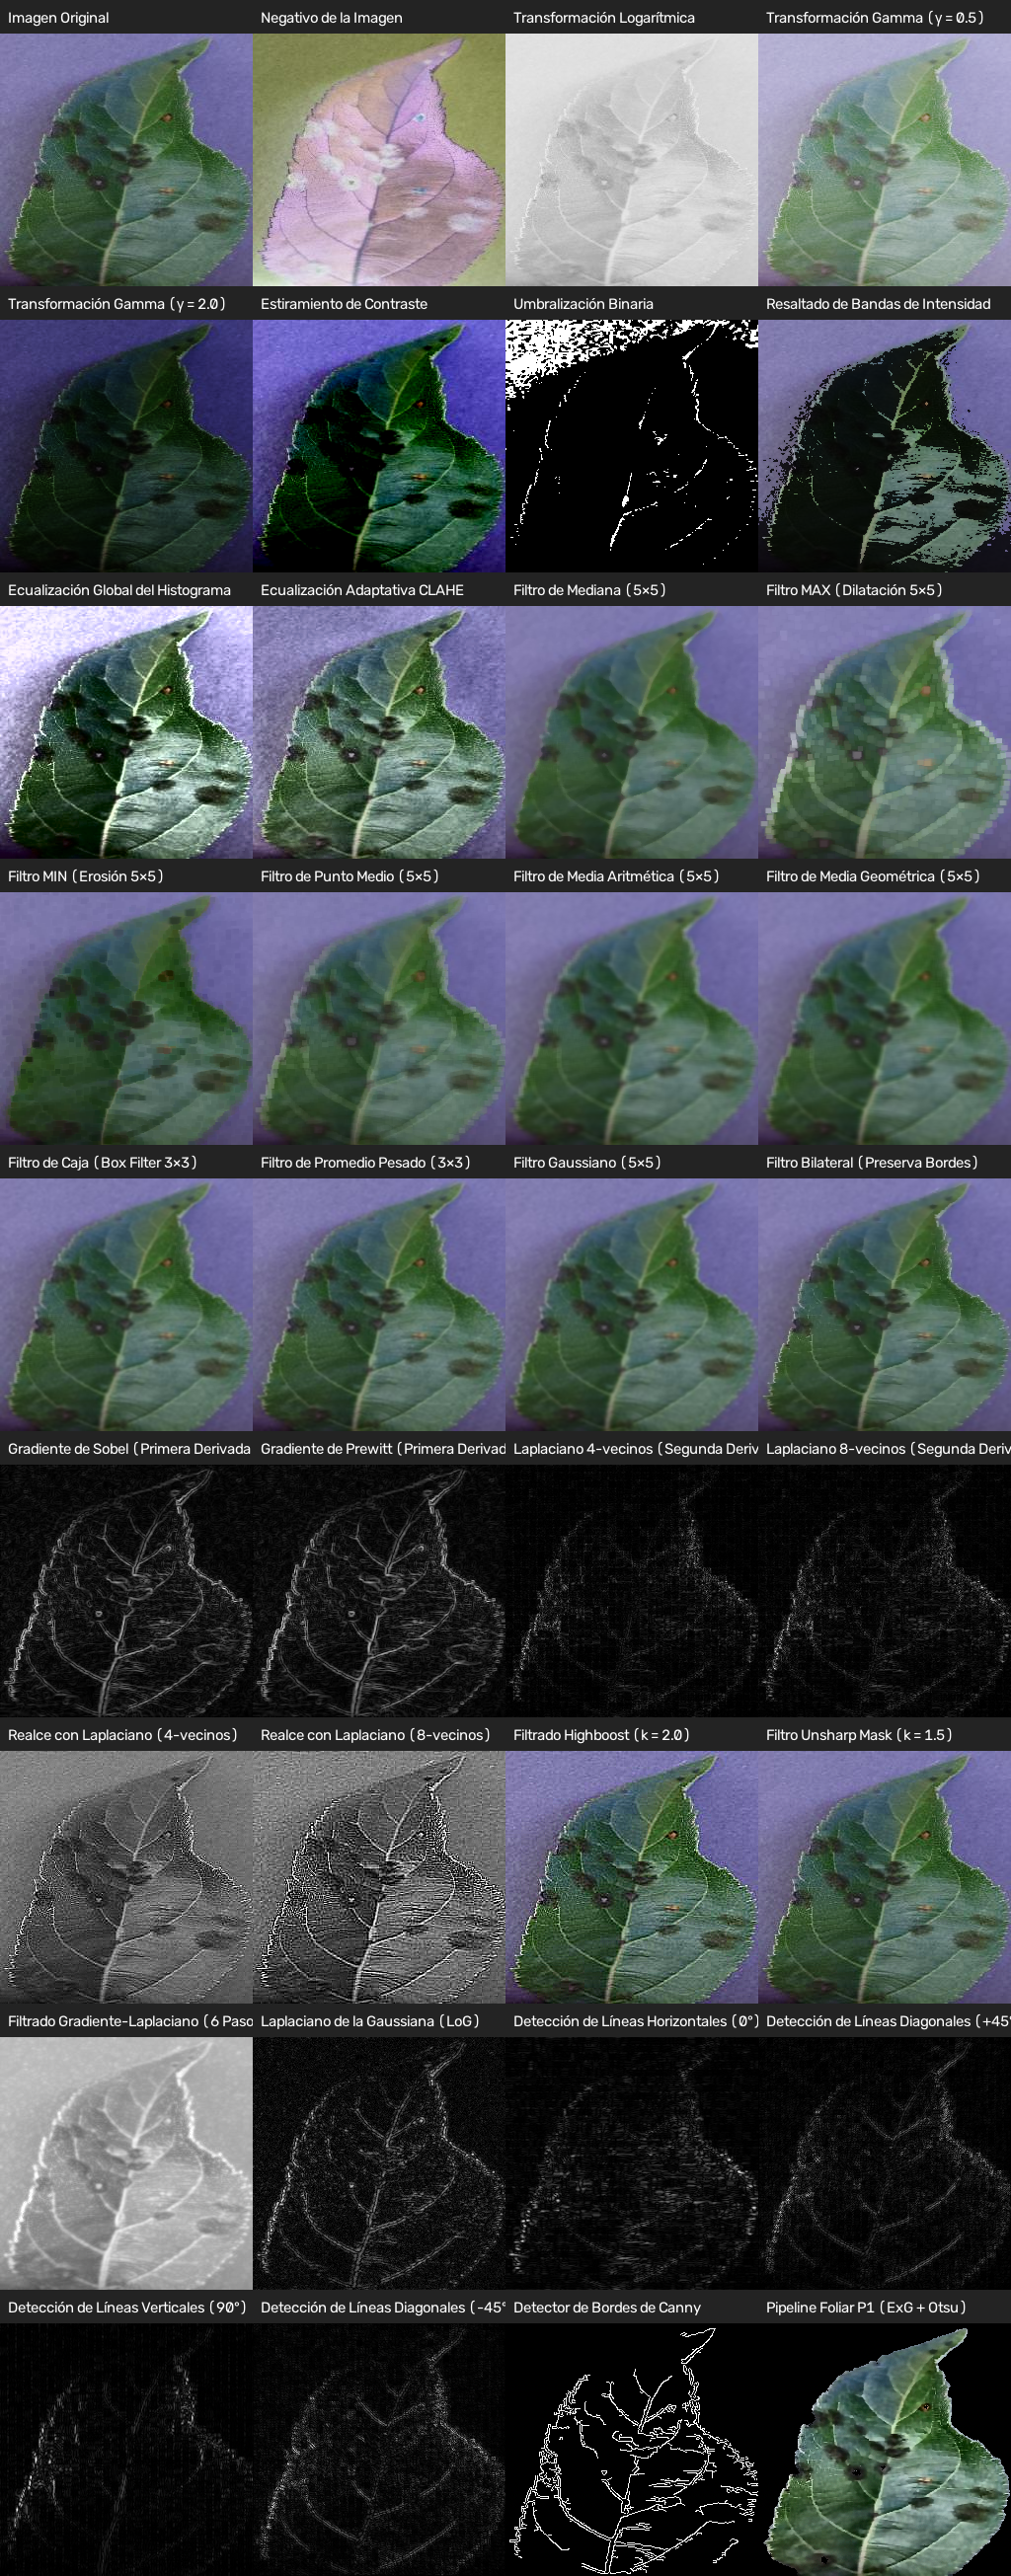
\includegraphics[
        width=\textwidth,
        height=0.72\textheight,
        keepaspectratio
    ]{resultados/filtros_02.png}
    \caption{Comparación de filtros aplicada a la segunda imagen de muestra.}
    \label{fig:comparacion2}
\end{figure}

\begin{figure}[p]
    \centering
    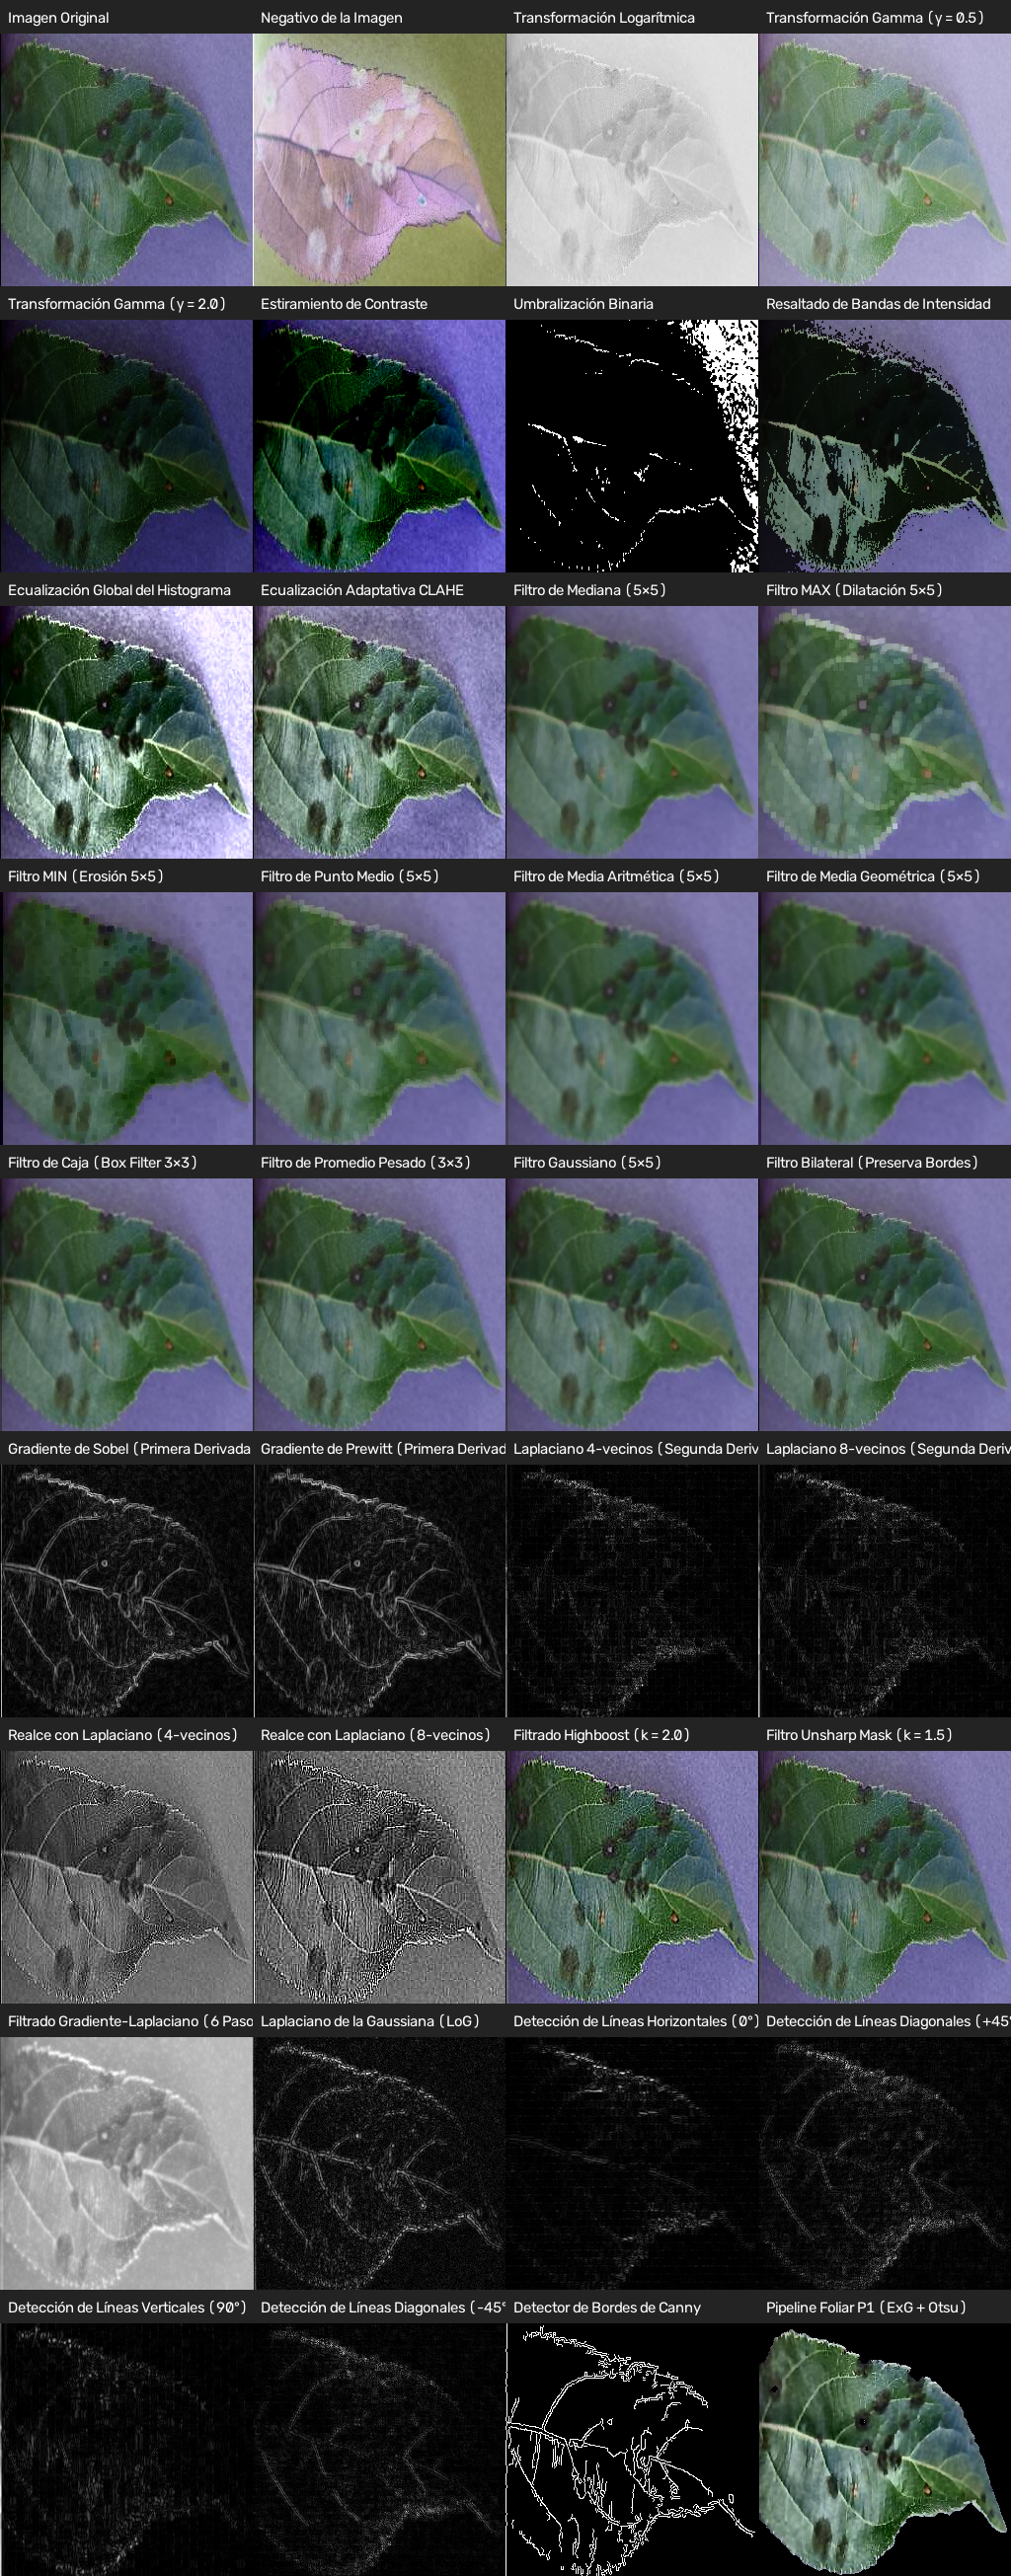
\includegraphics[
        width=\textwidth,
        height=0.72\textheight,
        keepaspectratio
    ]{resultados/filtros_03.png}
    \caption{Comparación de filtros aplicada a la tercera imagen de muestra.}
    \label{fig:comparacion3}
\end{figure}

\clearpage

\textbf{¿Cuál fue la mejor combinación de filtros?}

La combinación más efectiva fue usar primero el \textit{Filtro de mediana} para limpiar el ruido,
luego la \textit{Ecualización CLAHE} para mejorar el brillo y finalmente el \textit{Filtro Unsharp}
para reforzar los bordes. Esta combinación supera a usar un solo filtro por las siguientes razones:

\begin{itemize}
    \item Filtros como el de \textit{Mediana} eliminan el ruido, pero al mismo tiempo pueden borrar
    textura importante de la hoja si se usan demasiado agresivamente.
    \item Al combinar técnicas, la imagen resultante conserva el aspecto natural de la hoja,
    mejora la visibilidad de las manchas y lesiones, y reduce la distracción del fondo.
    \item El resultado final es una imagen más uniforme y útil para clasificación o análisis posterior.
\end{itemize}

\subsection{Resultados Individuales por Filtro con Pie de Página}
Para el cumplimiento exhaustivo de la rúbrica del curso, el pipeline implementa la exportación individual de cada uno de los 36 filtros evaluados (clasificados en las 5 categorías canónicas de Gonzalez \& Woods: transformaciones de intensidad, filtros de orden estadístico, filtros suavizantes pasabajas, filtros de derivada y detectores de bordes avanzados). Cada imagen individual se renderiza como una tarjeta autocontenida que integra en su pie de página:
\begin{enumerate}
    \item \textbf{Encabezado de Categoría y Título:} Nombre canónico del filtro.
    \item \textbf{Ecuación / Kernel matemático:} Formulación analítica formal ($s = T(r)$ o convolución discreta).
    \item \textbf{Propósito y Análisis Teórico:} Explicación cuantitativa del tipo de ruido atenuado, preservación de fronteras o realce de frecuencias espaciales.
\end{enumerate}
Los archivos individuales se encuentran organizados en \texttt{parcial1/resultados/individuales/muestra\_01/} a \texttt{muestra\_03/}, junto con el archivo auxiliar \texttt{figuras\_filtros.tex} para su inclusión directa en reportes extensos.

%--------------------------------------------------------------
\section{Referencias}
%--------------------------------------------------------------
\begin{thebibliography}{9}
\bibitem{gonzalez}
Gonzalez, R. C., \& Woods, R. E. (2018). \textit{Digital Image Processing} (4th ed.). Pearson.
\bibitem{kaggle}
Vipoooool. \textit{New Plant Diseases Dataset}. Kaggle. Disponible en: \url{https://www.kaggle.com/datasets/vipoooool/new-plant-diseases-dataset}
\bibitem{clahe}
Zuiderveld, K. (1994). Contrast Limited Adaptive Histogram Equalization. \textit{Graphics Gems IV}. Academic Press.
\end{thebibliography}

\end{document}
